%----------------------------------------------------------------------------------------
% CHAPTER TWO
%----------------------------------------------------------------------------------------
\chapter{THEORETICAL FOUNDATIONS} 
\label{ch:ch2}
%%%%%%%%%%%%%%%%%%%%%%%%%%%%%%%%%%%%%%%%%%%%%%%%%%%%%%%%%%%%%%%%%%%%%%%%%%%%%%%%%%%
\section{Crystallography Properties}
%%%%%%%%%%%%%%%%%%%%%%%%%%%%%%%%%%%%%%%%%%%%%%%%%%%%%%%%%%%%%%%%%%%%%%%%%%%%%%%%%%%
The hexagonal lattice nanostructure, a fundamental Bravais lattice, manifests as a distinctive geometric arrangement prevalent across a spectrum of materials, owing to its highly efficient packing characteristics. This lattice's spatial configuration profoundly influences the mechanical, electrical, and thermal properties of materials. Understanding lattice structures is crucial for deciphering material behavior across diverse conditions, spanning from semimetals to topological insulators. This significance is particularly noteworthy in the realm of two-dimensional materials. We have selected graphene, exemplifying a semimetal, and hexagonal boron nitride (h-BN), recognized as an insulator, for our discussion on nonlinear optical response on 2d materials.\\
\begin{figure}[htpb]
    \centering
    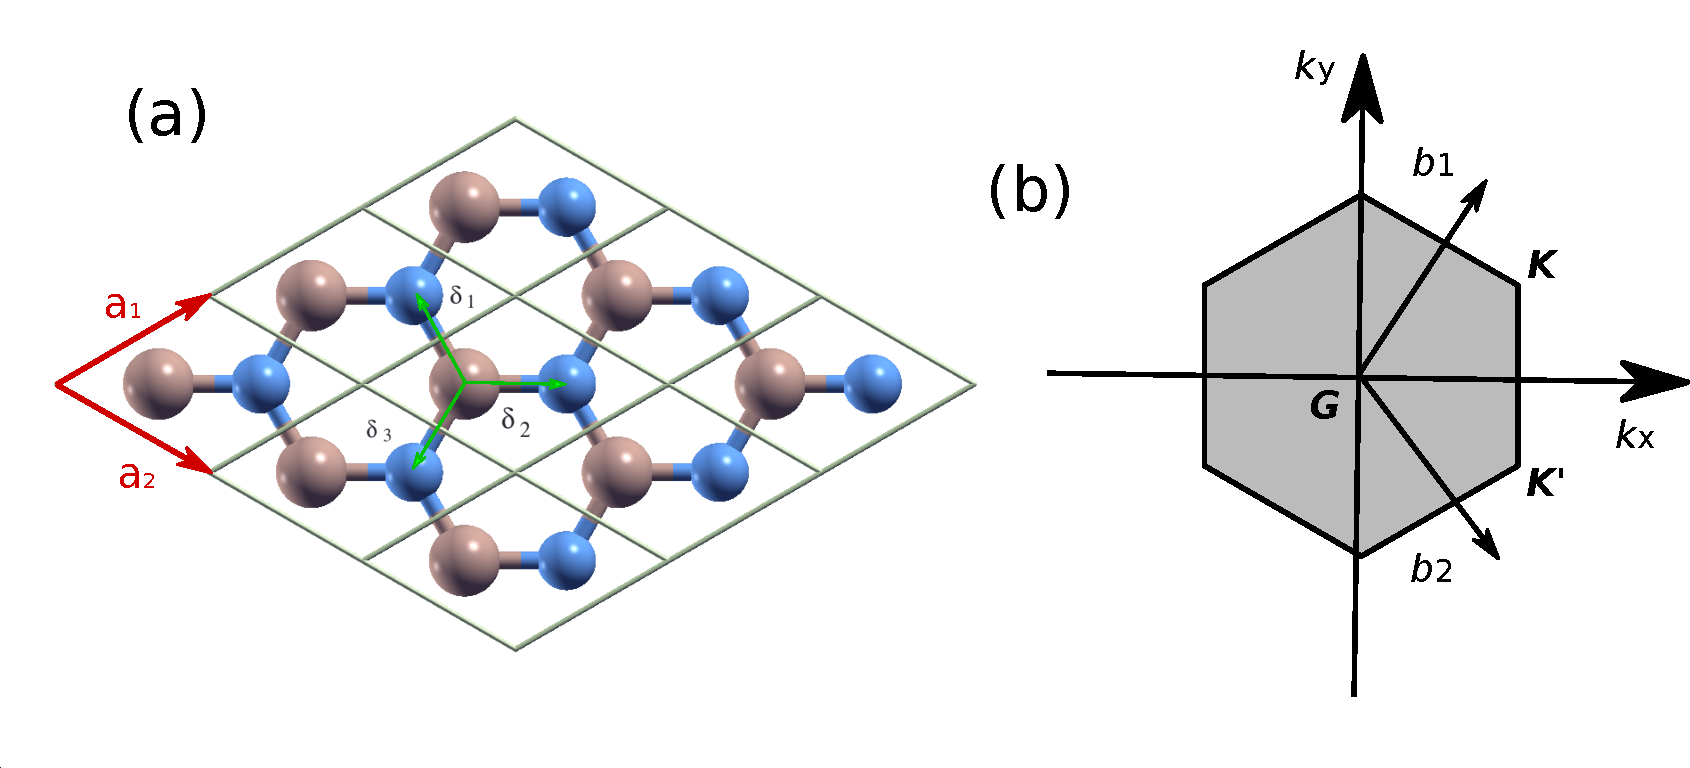
\includegraphics[width=0.96\textwidth]{pic/lattice.pdf}
    \caption[Lab coordinate system]{(a) Hexagonal lattice showing in different colors the two triangular sublattices. (b) Brillouin zone in momentum space.}
    \label{fig: lattice}
\end{figure}
Graphene, an extraordinary carbon allotrope, showcases a captivating atomic arrangement within a hexagonal lattice nanostructure, depicted in Figure \ref{fig: lattice} (a). Carbon atoms meticulously align in a single layer, forming an exceptional two-dimensional material. The unique atomic-scale hexagonal lattice structure involves each carbon atom intricately bonding through $\sigma$-bonds with its three nearest neighbors and a delocalized $\pi$-bond. This precise arrangement plays a pivotal role in the formation of a valence band elegantly spanning the entirety of the graphene sheet, making monolayer graphene an outstanding conductor of electricity, and finding applications in electronic devices, sensors, and various fields.

Similar to graphene, Hexagonal boron nitride (\gls{h-BN}) also features a hexagonal lattice structure, but with alternating boron and nitrogen atoms forming the hexagons, making it a wide-gap insulator due to inversion symmetry breaking, which is used as a dielectric material in electronics, a substrate for graphene-based devices, and as a solid lubricant.
% Example Subsubsection
\subsection{Structural Parameters}
% begin{figure}[tb] % t = top, b = bottom, etc.
 We define the basis of hexagonal lattice primitive vectors $E = (\vec{a}_{1}, \vec{a}_{2})$ as shown in Fig \ref{fig: lattice} (a):
$$
\vec{a}_{1}=a\left(\begin{array}{l}
\frac{\sqrt{3}}{2} \\
\frac{1}{2}
\end{array}\right),
\vec{a}_{2}=a\left(\begin{array}{l}
\frac{\sqrt{3}}{2} \\
-\frac{1}{2}
\end{array}\right)
$$
Where $a$ is the lattice constant, for graphene $a= 1.42 \mathring{A}$ \cite{sarma2011electronic}, and for \gls{h-BN} $a= 2.5 \mathring{A}$ \cite{PhysRevB.81.155433}. Generate only $A$ sites while sites in $B$ sublattice are generated by $n_{1} \vec{a}_{1}+n_{2} \vec{a}_{2}+\vec{\delta},$ where $\vec{\delta}$ has to be chosen as one of the three nearest-neighbor vectors,
$$
\begin{array}{c}
\vec{\delta}_{1}=a\left(\begin{array}{l}
-\frac{1}{2 \sqrt{3}}\\ \frac{1}{2}\end{array}\right), 
\vec{\delta}_{2}=a\left(\begin{array}{l}\frac{1}{\sqrt{3}}\\ 0 \end{array}\right),
\vec{\delta}_{3}=a\left(\begin{array}{l} -\frac{1}{2 \sqrt{3}}\\ -\frac{1}{2}\end{array}\right)
\end{array}
$$
\subsection{Reciprocal Space}
The reciprocal basis $B=\left(b_{1}, b_{2}, b_{3}\right)$ is generated using the formula:
$$
\overrightarrow{b_{k}}=\frac{2 \pi \cdot \overrightarrow{a_{i}} \times \overrightarrow{a_{j}}}{V}
$$
$i, j, k$ are circular permutations, $\mathrm{V}$ the mix product between the three vectors, i.e. the volume of the unitary cell.  Then we get the $2 \mathrm{D}$ reciprocal vectors as shown in Fig\ref{fig: lattice} (b):
$$
\vec b_{1}=k_{D}\left(\begin{array}{l}
\frac{1}{2} \\
\frac{\sqrt{3}}{2} 
\end{array}\right),
\vec b_{2}=k_{D}\left(\begin{array}{c}
\frac{1}{2} \\
-\frac{\sqrt{3}}{2} 
\end{array}\right)
$$
And with $k_{D}=\frac{4 \pi}{\sqrt{3} a}$. The corresponding Brillouin zone is depicted together with the two high-symmetry points $\mathrm{K}$ and $\mathrm{K'}$ Fig ~\ref{fig: lattice} (b).
Two inequivalent corners of the Brillouin zone $K$ and $K^{\prime}$ can be chosen as follows:
$$
K=k_{D}\left(\frac{1}{2}, \frac{1}{2 \sqrt{3}}\right), \quad K^{\prime}=k_{D}\left(\frac{1}{2},-\frac{1}{2 \sqrt{3}}\right)
$$

%%%%%%%%%%%%%%%%%%%%%%%%%%%%%%%%%%%%%%%%%%%%%%%%%%%%%%%%%%%%%%%%%%%%%%%%%%%%%%%%%%%
\section{Tight-binding Approach \label{sec:tightbinding}}
%%%%%%%%%%%%%%%%%%%%%%%%%%%%%%%%%%%%%%%%%%%%%%%%%%%%%%%%%%%%%%%%%%%%%%%%%%%%%%%%%%%

In this section, we delve into the fundamental principles of the tight-binding approach, with a particular focus on the nearest neighbor tight-binding model. This approach is essential for understanding the electronic properties of materials and is a crucial component of graphene's electronic structure analysis.

The foundation of the tight-binding approach is rooted in the Bloch theorem, which is satisfied by the tight-binding function
\begin{equation}
\Phi_{\alpha}(\mathbf{r}, \mathbf{k})=\frac{1}{\sqrt{N}} \sum_{\mathbf{R}} e^{i \mathbf{k} \cdot \mathbf{R}} \phi_{\alpha}\left(\mathbf{r}-\mathbf{R}_{\alpha}\right), \alpha=A \text { or } B
\label{eqn:Bloch}
\end{equation}
Here, $N$ represents the number of unit cells, and $\phi_{\alpha}(\mathbf{r} - \mathbf{R}_{\alpha})$ denotes the orbital function of an electron at cell $\mathbf{R}$ in sublattice $\alpha$.
In the context of a honeycomb lattice, we focus on the nearest neighbor approximation. This approximation asserts that an atom in sublattice A only interacts with its three closest neighbor atoms in sublattice B. This simplification is particularly useful for understanding the interactions between electrons bound to non-equivalent atoms.

The Hamiltonian operator for this nearest-neighbor interaction is expressed as:
\begin{align}
\hat{H}_{A B}=\frac{1}{N} \sum_{\mathbf{R}_{A}} \sum_{\mathbf{R}_{B}} e^{i \mathbf{k}\left(\mathbf{R}_{B}-\mathbf{R}_{A}\right)}\left\langle\phi_{A}\left(\mathbf{r}-\mathbf{R}_{\mathbf{A}}\right)|\hat H| \phi_{B}\left(\mathbf{r}-\mathbf{R}_{B}\right)\right\rangle
\end{align}
Due to the translational invariance in a Bravais lattice, the summation over each atom in a sublattice occurs $N$ times, simplifying the expression to:
\begin{align}
\hat{H}_{A B}=\sum_{\mathbf{R}_{A}} e^{i \mathbf{k}\left(\mathbf{R}_{B}-\mathbf{R}_{A}\right)}\left\langle\phi_{A}\left(\mathbf{r}-\mathbf{R}_{\mathbf{A}}\right)|\hat{H}| \phi_{B}\left(\mathbf{r}-\mathbf{R}_{B}\right)\right\rangle
\end{align}
To transition from real space to momentum space, we employ a Fourier transform, allowing us to represent the Hamiltonian in terms of momentum space. This transformation results in the tight-binding Hamiltonian under the momentum representation, as defined by:
\begin{align}
c_{ \mathbf{R}_{\alpha}, \sigma}=\frac{1}{\sqrt{N}} \sum_{\mathbf{k}} e^{i \mathbf{k} \cdot 
 \mathbf{R}_{\alpha}} c_{\mathbf{k}, \sigma} \\
 c_{\mathbf{R}_{\alpha}, \sigma}^{\dagger}=\frac{1}{\sqrt{N}} \sum_{\mathbf{k}} e^{-i \mathbf{k} \cdot \mathbf{R}_{\alpha}} c_{\mathbf{k}, \sigma}^{+}
 \label{eqn: FT}
\end{align}
 $\sigma=\uparrow, \downarrow$ presents the electron spin,
 With the  orthogonal normalization conditions 
 \begin{align}
   \delta_{\mathrm{kk}^{\prime}}=\frac{1}{N} \sum e^{i\left(k-k^{\prime}\right) \cdot \mathrm{R}_{\alpha}}  
 \end{align}
 We transform the Hamiltonian of real space into the momentum space representation, and then the tight-binding Hamiltonian under the momentum representation is:
\begin{equation}
\hat{H} =\left(\begin{array}{cc}
\epsilon_{A} & t_{0} f(\mathbf{k}) \\
t_{0} f(\mathbf{k})^{*} & \epsilon_{B}
\end{array}\right)
\label{eqn: TBh}
\end{equation}

Here $\epsilon_{A}$ and $\epsilon_{B}$ are the on-site energies of electrons on the nearest neighbor atoms, $t_0$ presents the hopping parameter:
$$
t_{0}=\left\langle\phi_{A}\left(\mathbf{r}-\mathbf{R}_{\mathbf{A}}\right)|\hat{H}| \phi_{B}\left(\mathbf{r}-\mathbf{R}_{A}-\vec{\delta}_{i}\right)\right\rangle \quad(i=1,2,3)
$$\\
For graphene, we set $\epsilon_{A}$ and $\epsilon_{B}$ to 0, and $t_0=2.8~eV$ in accordance with the previous work  \cite{sarma2011electronic}. For h-BN $\epsilon_{\mathrm{B}}$ and $\epsilon_{\mathrm{N}}$ denote the on-site energies for boron and nitrogen sites, respectively. 
\begin{equation}
\hat{H}(\mathbf{k})=\left(\begin{array}{cc}
\epsilon_{\mathrm{B}} & t_{0} f(\mathbf{k}) \\
t_{0} f(\mathbf{k})^{*} & \epsilon_{\mathrm{N}}
\end{array}\right),
\label{eqn:hBNhamiltonian}
\end{equation}
We set $\epsilon_{\mathrm{B}}$ to $3.34$~eV and $\epsilon_{\mathrm{N}}$ to $-2.56~eV$ and $t0$ to $2.6~eV$ computed with the first-principles calculations~\cite{PhysRevB.51.6868}, the band gap $E_{g}=\epsilon_{b}-\epsilon_{n}$ equals 5.9~eV. 

The off-diagonal terms of the tight-binding Hamiltonian \ref{eqn: TBh}:
\begin{equation}
 \begin{aligned}
f(\mathbf{k}) &=e^{i \mathbf{k} \vec{\delta}_{1}}+e^{i \mathbf{k} \vec{\delta}_{2}}+e^{i \mathbf{k} \vec{\delta}_{3}} \\
&=e^{-\frac{i a k_{x}}{\sqrt{3}}}+2 e^{\frac{i a k_{x}}{2 \sqrt{3}}} \cos \left(\frac{a}{2} k_{y}\right)
\end{aligned}
\label{eqn:nearest_h}
\end{equation}
Solving the stationary Schrödinger equation using matrix diagonalization:
\begin{align}
\hat{H}_{\vecb{k}}|\phi_{b \vecb{k}}\rangle = \epsilon_{b\vecb{k}}|\phi_{b}\rangle,
\label{eq:eqigenstates-h0}
\end{align}
We get the eigenenergy of Hamiltonian from \ref{eqn: TBh}, where $b$ is a band index, $|\phi_{b\vecb{k}}\rangle$ is an eigenstate, and $\epsilon_{b\vecb{k}}$ corresponds to the eigenenergy. As the Hamiltonian is a $2$-by-$2$ matrix in this work, the band index $b$ denotes either a conduction ($b=c$) or valence ($b=v$) state.

\begin{equation}
\epsilon_{b\vecb{k}}=E_{0} \pm \frac{1}{2} \sqrt{E_{g}^{2}+4t_{0}^{2}|f|^{2}}
\label{eigenvalues}
\end{equation}
$E_{0}=\frac{\epsilon_{A}+\epsilon_{B}}{2}$ and $E_{g}=\epsilon_{b}-\epsilon_{n}$ is the energy gap. For graphene, $\epsilon_{A} = \epsilon_{B} =0$ the band gap equals 0.
Their corresponding eigenvectors are:
\begin{equation}
    |\phi_{b}\rangle  =\left(\begin{array}{cc}
 \frac{E_{g} \pm \sqrt{E_{g}^{2}+4t_{0}^{2}|f|^{2}}}{2t_{0} f^*}\\
1
\end{array}\right)
\label{eqn:eigenvector}
\end{equation}

%%%%%%%%%%%%%%%%%%%%%%%%%%%%%%%%%%%%%%%%%%%%%%%%%%%%%%%%%%%%%%%%%%%%%%%%%%%%%%%%%%%
\section{Electron Dynamics}
%%%%%%%%%%%%%%%%%%%%%%%%%%%%%%%%%%%%%%%%%%%%%%%%%%%%%%%%%%%%%%%%%%%%%%%%%%%%%%%%%%%
Consider the crystal under the electric field $\vecb {E}$, to avoid that
Bloch’s theorem cannot be applied, let the electric field enter through a uniform vector potential $\vecb {A} (t)$. The time-dependent Hamiltonian is written as
\begin{align}
\hat{H}(t)=\frac{[\hat{\boldsymbol{p}}+e \boldsymbol{A}(t)]^{2}}{2 m}+V(\boldsymbol{r})
\end{align}
Transforming to the $\boldsymbol{k}$ -space representation, we have
\begin{equation}
     \hat{H}(\boldsymbol{k}, t)=\hat{H}\left(\boldsymbol{k}+\frac{e}{\hbar} \boldsymbol{A}(t)\right)
     \label{eqn:vTD}
\end{equation}
where $\boldsymbol k$ denotes the Bloch wavevector, and $|\psi_{\boldsymbol k}(t)\rangle$ is a single-particle electroinc wavefunction at $\boldsymbol k$. The vector potential $\vecb A(t)$ is related to the applied electric field $\vecb E(t)$ as $\vecb E(t)=-d\vecb A(t)/dt$, and it is included in the Hamiltonian as the wavevector shift $\boldsymbol k \rightarrow \boldsymbol k + e\vecb A(t)/\hbar$ via the Peierls substitution  \cite{hofstadter1976energy}.\\
%===================================================================================================================================
\subsection{Time-dependent Schr\"odinger Equation}
The light-induced electron dynamics can be described by solving the following time-dependent Schr\"odinger equation (\gls {TDSE}) at each $\vecb k$-point:
\begin{equation}
i\hbar \frac{d}{dt}| \psi_{\boldsymbol {k}}(t) \rangle = \hat{H}\left ( \boldsymbol k + \frac{e\vecb A(t)}{\hbar} \right )| \psi_{\boldsymbol k}(t) \rangle,
\label{eqn:TDSE}
\end{equation}
Solving this time-dependent Schr\"odinger equation (\gls {TDSE}) is an initial value problem. In two-band systems, usually the ground state $\psi_{\boldsymbol k}(0)$ is used as the initial state occupied at the valence band with:
\begin{align}
\psi_{\boldsymbol k}(0) = \left(\begin{array}{cc}
0 \\
1
\end{array}\right)
\end{align}
The adiabatic approximation is used almost all the time in solving time-propagation, which will be explained in more detail in the appendix \ref{sec:A_ADIABATIC}. Various numerical schemes can be chosen for doing the time propagation, here we split the propagation into short-time propagation using the composition property:
\begin{equation}
\left|\psi_{\boldsymbol{k}}(t')\right\rangle=\exp \left[-i \int_{t}^{t'} d \tau \hat{H}(\tau) \right]\left|\psi_{\boldsymbol{k}+\vecb{A}(t)}\right\rangle
\label{eqn:Houston}
\end{equation}
In practice, simpler schemes are usually used and self-consistency is often neglected. Instead, we rely on a sufficiently small $\Delta t$, $t'=t+\Delta t$, the exponential mid-point propagator is given by:
\begin{align}
    U(t+\Delta t, t) \approx U_{E M}(t+\Delta t, t)=\exp \{-\mathrm{i} \Delta t \hat{H}(t+\Delta t / 2)\}
\end{align}
We approximate the exponential using a Taylor expansion to fourth-order:
\begin{align}
    \exp \{A\}=\sum_{k=0}^{\infty} \frac{1}{k!} A^k
\end{align}
Once the time-evolution of the wavefunctions, $|\psi_{\vecb k}(t)\rangle$ is computed, the current induced in the matter can be further evaluated with
\begin{align}
\vecb{J}_{\vecb k}(t)=\frac{1}{(2\pi)^2} \int_{BZ} d\vecb k\langle \psi_{\vecb k}(t)|\hat{\vecb J}_{\vecb k}(t)| \psi_{\vecb{k}}(t)\rangle.
\label{eq:current}
\end{align}
Here, $\hat {\vecb J}_{\vecb k}(t)$ is the current operator, and it is defined as
\begin{align}
\hat {\vecb J}_{\vecb k}(t) = \frac{\partial }{\partial \vecb k}\hat H \left (\vecb k + \frac{e\vecb A(t)}{\hbar} \right ) = 
-t_0 \left(\begin{array}{cc}
0 & \frac{\partial f(\boldsymbol{k}+\boldsymbol{A})}{\partial \boldsymbol A} \\
\frac{\partial f^*(\boldsymbol{k}+\boldsymbol{A})}{\partial \boldsymbol A}  & 0
\end{array}\right),
\end{align}

where $\frac{\partial f(\vecb k)}{\partial \vecb k}$ is given by 
\begin{align}
\frac{\partial f(\vecb k)}{\partial \vecb k}=i \vecb{\delta}_1e^{i\vecb k \cdot \vecb \delta_1}
+i \vecb{\delta}_2e^{i\vecb k \cdot \vecb \delta_2}
+i \vecb{\delta}_3e^{i\vecb k \cdot \vecb \delta_3}.
\end{align}
Current \ref{eq:current} can be further decomposed into:
\begin{equation}
\begin{array}{l}
\boldsymbol{J}_{b,k}(t)=\left\langle \psi_{b, \boldsymbol{k}}(t)|\boldsymbol{J}(t))| \psi_{b, \boldsymbol{k}}(t)\right\rangle \\
=\sum\limits_{b',b''} c_{b^{\prime} \boldsymbol{k}}(t) c_{b^{\prime \prime} \boldsymbol{k}}^{*}(t)\left\langle \phi_{b^{\prime \prime} \boldsymbol{k}}^{H}(t)|\boldsymbol{J}(t))| \phi_{b^{\prime} \boldsymbol{k}}^{H}(t)\right\rangle+\sum\limits_{b',b''}\left|c_{b^{\prime} k}(t)\right|^{2}\left\langle \phi_{b^{\prime} k}^{H}(t)|\boldsymbol{J}(t))| \phi_{b^{\prime} k}^{H}(t)\right\rangle
\end{array}
    \label{totalcurrent}
\end{equation}
Here the off-diagonal terms contribute to the Interband current, and the diagonal terms contribute to the Intraband current. \\
\begin{equation}
\begin{array}{l}
\boldsymbol{J}_{inter;b,k}(t)=\sum\limits_{b',b''} c_{b^{\prime} \boldsymbol{k}}(t) c_{b^{\prime \prime} \boldsymbol{k}}^{*}(t)\left\langle \phi_{b^{\prime \prime} \boldsymbol{k}}^{H}(t)|\boldsymbol{J}(t))| \phi_{b^{\prime} \boldsymbol{k}}^{H}(t)\right\rangle
\end{array}
    \label{intercurrent}
\end{equation}

\begin{equation}
\begin{array}{l}
\boldsymbol{J}_{intra;b,k}(t)=\sum\limits_{b',b''}\left|c_{b^{\prime} k}(t)\right|^{2}\left\langle \phi_{b^{\prime} k}^{H}(t)|\boldsymbol{J}(t))| \phi_{b^{\prime} k}^{H}(t)\right\rangle
\end{array}
    \label{intracurrent}
\end{equation}
By combining time-dependent wavefunction $\psi_{\vecb{k}}(t)$ solved from Eq.~(\ref{eqn: TBh}) and the eigenstates $\phi_{c\vecb{k}}$ defined with Eq.~(\ref{eq:eqigenstates-h0}), the conduction population distribution $n_{c \vecb{k}}$ with the laser irradiation at instantaneous time $t$  can be evaluated as:
\begin{equation}
  n_{c\vecb{k}} = \left | \langle \phi_{c\vecb{k}} | \psi_{\vecb{k}}(t) \right |^2,
  \label{eq:population_tdse}
\end{equation}
$\frac{\partial\epsilon_{b,\boldsymbol{k}+\boldsymbol{A}(t)}}{\partial\boldsymbol{k}} = -\left\langle \phi_{b^{\prime} k}^{H}(t)|\boldsymbol{J}(t))| \phi_{b^{\prime} k}^{H}(t)\right\rangle$ defines the band velocity. The eigenenergy of conduction band at time $t$ is $\epsilon_{c,\boldsymbol{k}+\boldsymbol{A}(t)}=E_{0} + \frac{1}{2} \sqrt{E_{g}^{2}+4t_{0}^{2}|f(\boldsymbol{k}+\boldsymbol{A}(t))|^{2}}$\\

\begin{equation}
    \frac{\partial\epsilon_{v,\boldsymbol{k}+\boldsymbol{A}(t)}}{\partial\boldsymbol{k}}=-\frac{t_0^2}{2\epsilon_{v,k+\boldsymbol{A}(t)}-(\epsilon_b+\epsilon_n)}\cdot (f^*(\boldsymbol{k}+\boldsymbol{A}(t))\frac{\partial f(\boldsymbol{k}+\boldsymbol{A}(t))}{\partial k}+c.c.)
    \label{band velocity_v}
\end{equation}

\begin{equation}
    \frac{\partial\epsilon_{c,\boldsymbol{k}+\boldsymbol{A}(t)}}{\partial\boldsymbol{k}}=\frac{t_0^2}{2\epsilon_{c,k+\boldsymbol{A}(t)}-(\epsilon_b+\epsilon_n)}\cdot (f^*(\boldsymbol{k}+\boldsymbol{A}(t))\frac{\partial f(\boldsymbol{k}+\boldsymbol{A}(t))}{\partial k}+c.c.)
    \label{band velocity_c}
\end{equation}
%==================================================================================================================================
\subsection{Quantum Master Equation \label{sec:master}}
In contrast to closed quantum systems, which are entirely isolated from external influences and can be adequately described by the Schrödinger equation, the quantum master equation is typically used in the context of the time evolution of an open quantum system, where the system of interest is susceptible to exchanges of energy, particles, or information with its external environment. 
To expound processes such as relaxation, dephasing, and thermalization of the nonlinear response experiments, the quantum master equation is predominantly employed which is salient in the realm of open quantum systems.\\
We describe the light-induced electron dynamics in graphene with the following quantum master equation \cite{sato2019light,sato2019microscopic,sato2021high,sato2021nonlinear}:
\begin{equation}
\frac{\mathrm{d}}{\mathrm{d}t}\rho_{\boldsymbol{k}}(t) = \frac{1}{i \hbar}	\left[ \hat{H}_{\boldsymbol{k}+e\boldsymbol{A}(t)/\hbar}, \rho_{\boldsymbol{k}} (t)) \right] + 	
\hat{D}\left[ \rho_{\boldsymbol{k}} (t)) \right],
\label{eqn:masterequation}
\end{equation}
$\rho_{\vecb k}(t)$ is the reduced density matrix at $\vecb k$. The quantum master equation delineates the dynamical evolution of the density matrix associated with the quantum system, which encompasses both pure and mixed quantum states. 
To elucidate the impact of dissipation, we formulate the relaxation operator, denoted as $\hat{D}\left[\rho_{\vecb{k}} (t)\right]$, within the framework of Eq.(\ref{eqn:masterequation}) employing the relaxation time approximation\cite{meier1994coherent} and employing the Houston basis \cite{PhysRev.57.184, PhysRevB.33.5494}. The Houston states are characterized as eigenstates of the instantaneous Hamiltonian, expressed as:
\begin{align}
\hat{H}_{\vecb{k}+e\vecb{A}(t)/\hbar} |u^H_{b\vecb k}(t)\rangle = \epsilon_{b,\vecb k + e\vecb A(t)/\hbar}|u^H_{b\vecb k}(t)\rangle   
\label{eqn:Houston}
\end{align}
The expansion of the reduced density matrix can then be carried out using the Houston states.
\begin{align}
  \rho_{\vecb k}(t) = \sum_{bb'}\rho_{bb',\vecb k}(t)|u^H_{b\vecb k}(t)\rangle \langle u^H_{b'\vecb k}(t)|,
\end{align}
where $\rho_{bb',\vecb k}(t)$ are the expansion coefficients. On the basis of the Houston state expansion, we define the relaxation operator \cite{sato2019microscopic,PhysRevB.99.214302,sato2019light} as
\begin{align}
    \hat D\left [\rho_{\vecb k}(t) \right ]=&-\sum_{b}\frac{\rho_{bb,\vecb k}(t)-f^{FD}\left
(\epsilon_{b,\vecb k+e\vecb A(t)/\hbar},T_e,\mu \right)}{T_1}|u^H_{b\vecb k}(t)\rangle \langle
u^H_{b\vecb k}(t)|\\ 
                                            &-\sum_{b\neq b'} \frac{\rho_{bb',\vecb k}(t)}{T_2}|u^H_{b\vecb k}(t)\rangle \langle u^H_{b'\vecb k}(t)|,
\label{eqn:relaxation}
\end{align}
$T_1$ is the longitudinal relaxation time, $T_2$ is the transverse relaxation time, and $f^{\mathrm{FD}}(\epsilon)$ is the Fermi--Dirac distribution
\begin{align}
f^{\mathrm{FD}}(\epsilon, T_e, \mu)=\frac{1}{e^{(\epsilon-\mu)/k_BT_e}+1}.
\label{eq:fd-dist}
\end{align}
$\mu$ is the chemical potential, and $T_e$ is the electron temperature.
In the following discussion, we set the longitudinal relaxation time $T_1$ to $100$~fs and the transverse relaxation time $T_2$ to $20$~fs in accordance with the previous works \cite{sato2021nonlinear,sato2021high,sato2019light,sato2019microscopic}. The electron temperature $T_e$ is set to $300$~K unless stated otherwise. The chemical potential $\mu$ is treated as a tunable parameter to study the effect of doping.\\
We directly solve the quantum master equation, Eq.~(\ref{eqn:masterequation}), in the time domain by employing the Runge-Kutta method without any approximation.
The electric current is obtained by employing the time-dependent density matrix $\rho_{\vecb k}(t)$, which evolves according to Eq.~(\ref{eqn:masterequation}):
\begin{eqnarray}
  \vecb{J}(t)=\frac{2}{(2\pi)^2} \int d\vecb k \mathrm{Tr}\left[\hat{\boldsymbol{J}}_{\boldsymbol{k}}(t)\rho_{\boldsymbol{k}}(t)\right],
\label{eqn:totalcurrent}
\end{eqnarray}
where $\hat{\boldsymbol{J}}_{\boldsymbol{k}}(t)$ is the current operator defined as
\begin{align}
\hat{\boldsymbol J}_{\boldsymbol{k}}(t) = -\frac{\partial H(\boldsymbol{k}+e\boldsymbol{A}(t)/\hbar)}{\partial \boldsymbol A(t)}.
\label{totalcurrent}
\end{align}
The intraband component of the current is
\begin{align}
\boldsymbol{J}^{\mathrm{intra}}_{\vecb k}(t)&=\sum_{b=v,c} \frac{(-2)}{(2\pi)^2}
\frac{e}{\hbar} \nonumber \times  
\int d\boldsymbol{k}\frac{\partial\epsilon_{b,\boldsymbol{k}+e\boldsymbol{A}(t)/\hbar}}{\partial\boldsymbol{k}} n_{b,\boldsymbol{k}+e\boldsymbol{A}(t)/\hbar},
\label{eqn:intra-steady-current}
\end{align}
where the band population $n_{b,\boldsymbol{k}+e\boldsymbol{A}(t)/\hbar}$ is defined with the Houston states of the Hamiltonian $|u^H_{b,\boldsymbol k} (t)\rangle$ computed from Eq ~\ref{eqn:Houston}:
\begin{align}
n_{b,\boldsymbol{k}+e\boldsymbol{A}(t)/\hbar}(t)=\langle u^H_{b,\boldsymbol k}(t) |\rho_{\boldsymbol{k}}(t)|u^H_{b,\boldsymbol k}(t) \rangle
\end{align}
%=====================================================================================================================================================


